\newsection

\subsection{BP 5:
 Solitary wave on composite beach (Laboratory) }


\subsubsection{Problem specification}

\begin{itemize}
\item PMEL-135, pp 6 \& 37-39.

\item Problem description provided by Elena Tolkova at
\cite{bp-description}:\\
\href{https://github.com/rjleveque/nthmp-benchmark-problems/blob/master/BP05-ElenaT-Solitary_wave_on_composite_beach_laboratory/BP5_description.pdf}
{BP05-ElenaT-Solitary\_wave\_on\_composite\_beach\_laboratory/BP5\_description.pdf} 

\item Coastal Hydraulics Laboratory Problem Description\cite{CHLBP2}
\end{itemize}

This is the same problem as in BP 2, but using the nonlinear shallow water
equations and comparing to laboratory data rather than to the analytic
solution of the linear equations.

\subsubsection{What we did}
\begin{itemize}
\item We solved the shallow water wave equation in Cartesian coordinates with $g = 9.81$ and no friction.
\item To specify the incoming wave from the left boundary of our
computational domain we used the first ten seconds of  measurements taken at
Gage 4.  After ten seconds the left boundary switched to be a non-reflecting
boundary.  This boundary is selected since the end of our computational
domain is not the end of the physical wave tank.  The implementation of
these boundary conditions is described in \Sec{bc}.
\item We solved on a $600 \times 2$ grid with no adaptive mesh refinement. 
\end{itemize}

\subsubsection{Gage comparisons}
The results for cases A, B, and C are shown in figures \Fig{bp5A}, \Fig{bp5B}, \Fig{bp5C} respectively where Gage 11 is placed at the vertical wall.

\begin{figure}[ht]
\hfil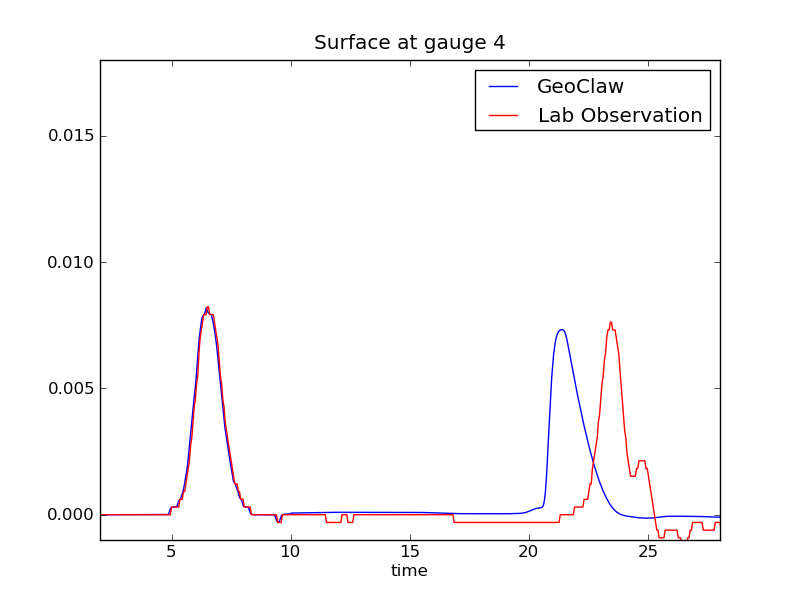
\includegraphics[width=2.8in]{bp5/CaseA/gauge0004fig300.png}\hfil
\hfil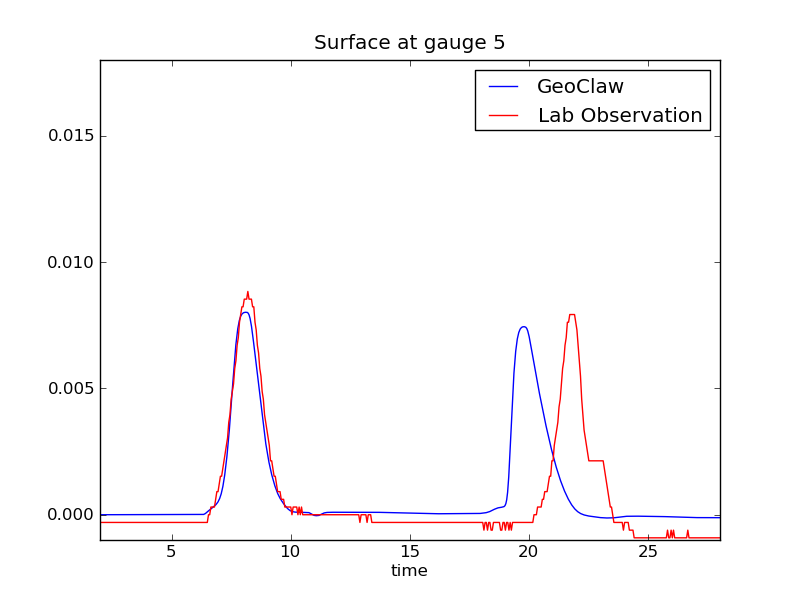
\includegraphics[width=2.8in]{bp5/CaseA/gauge0005fig300.png}\hfil
\vskip 5pt
\hfil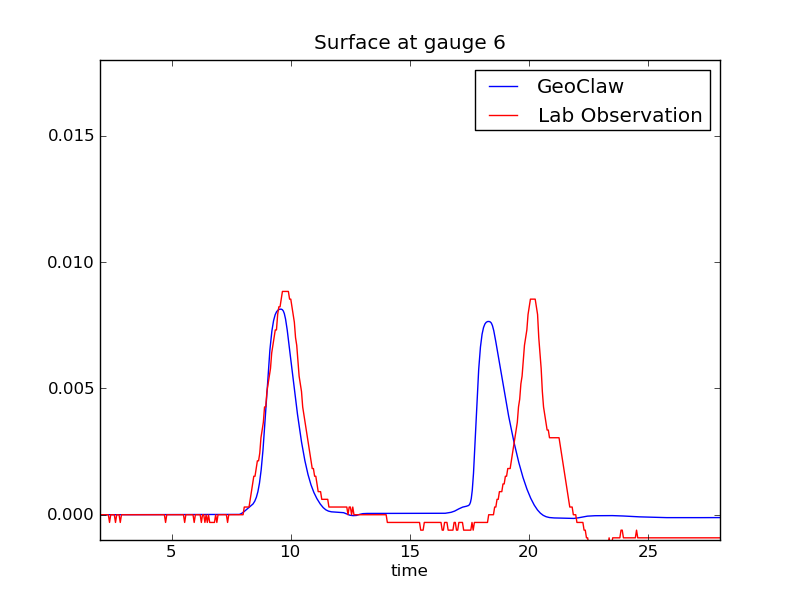
\includegraphics[width=2.8in]{bp5/CaseA/gauge0006fig300.png}\hfil
\hfil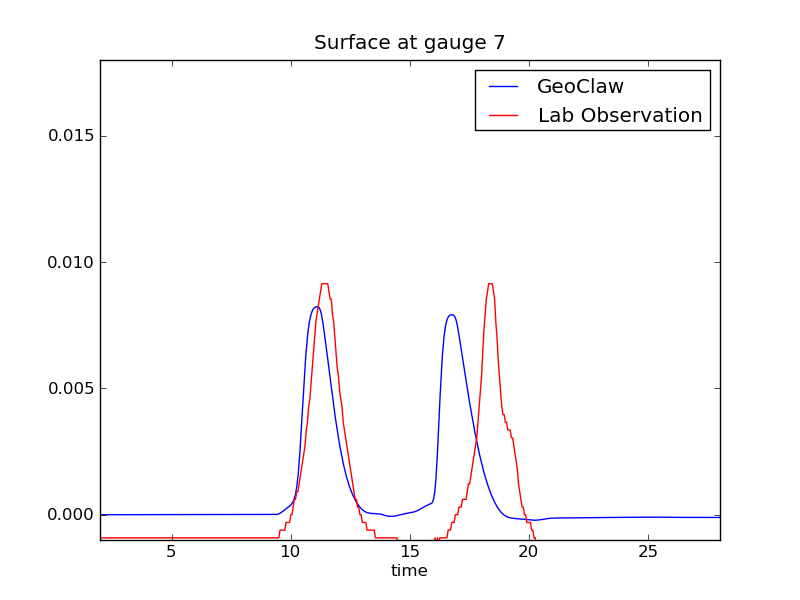
\includegraphics[width=2.8in]{bp5/CaseA/gauge0007fig300.png}\hfil
\vskip 5pt
\hfil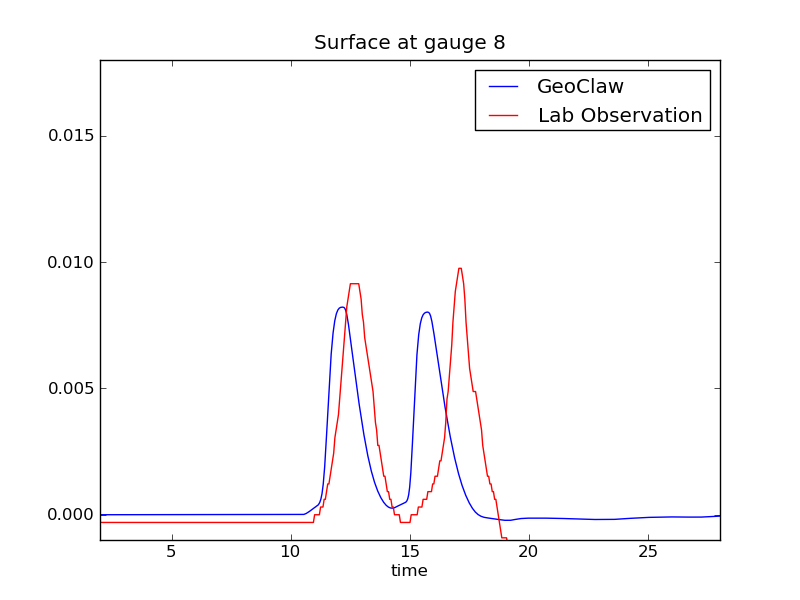
\includegraphics[width=2.8in]{bp5/CaseA/gauge0008fig300.png}\hfil
\hfil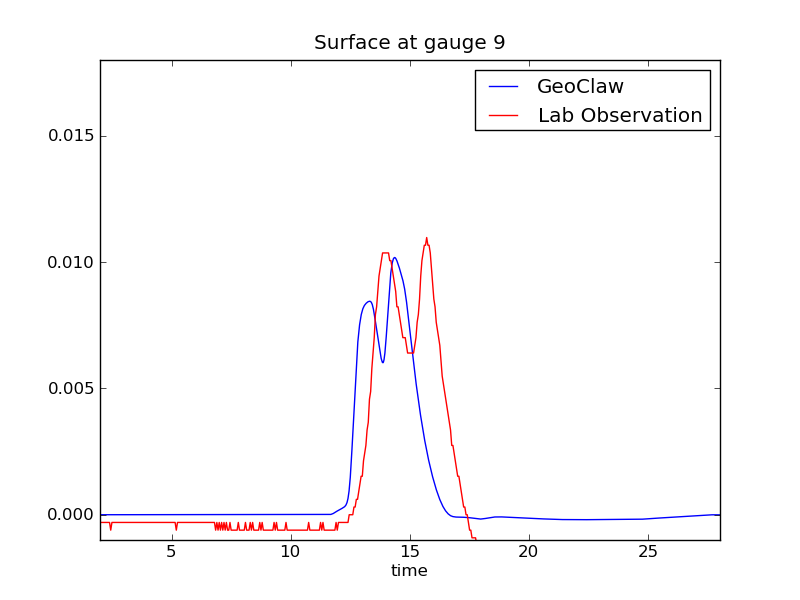
\includegraphics[width=2.8in]{bp5/CaseA/gauge0009fig300.png}\hfil
\vskip 5pt
\hfil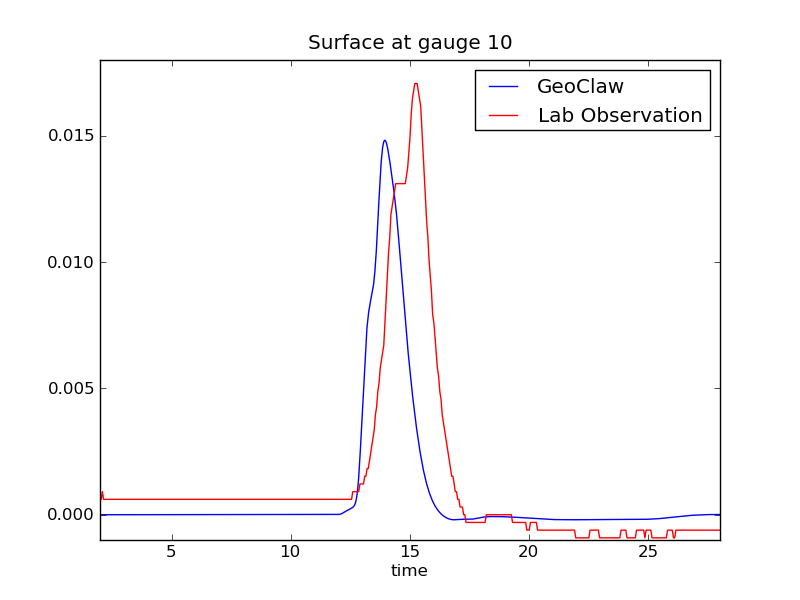
\includegraphics[width=2.8in]{bp5/CaseA/gauge0010fig300.png}\hfil
\hfil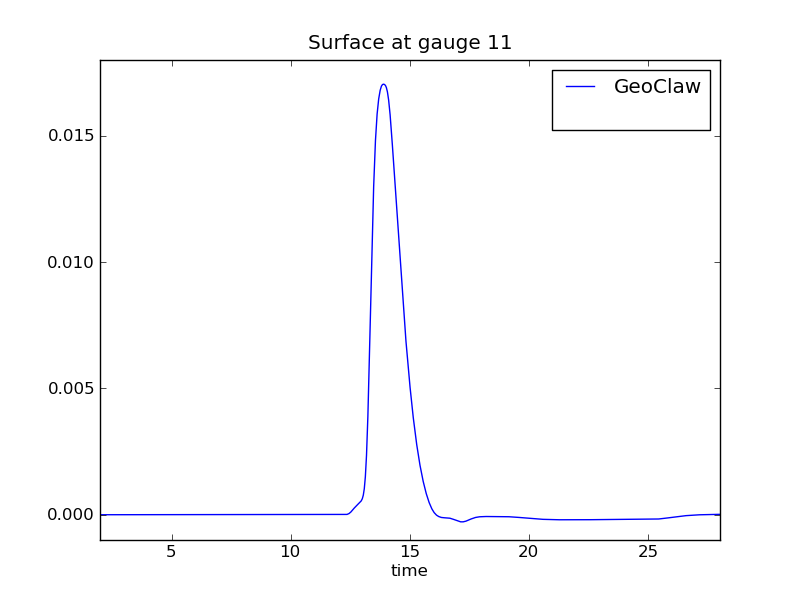
\includegraphics[width=2.8in]{bp5/CaseA/gauge0011fig300.png}\hfil
\caption{\label{fig:bp5A} Case A }
\end{figure}

\begin{figure}[ht]
\hfil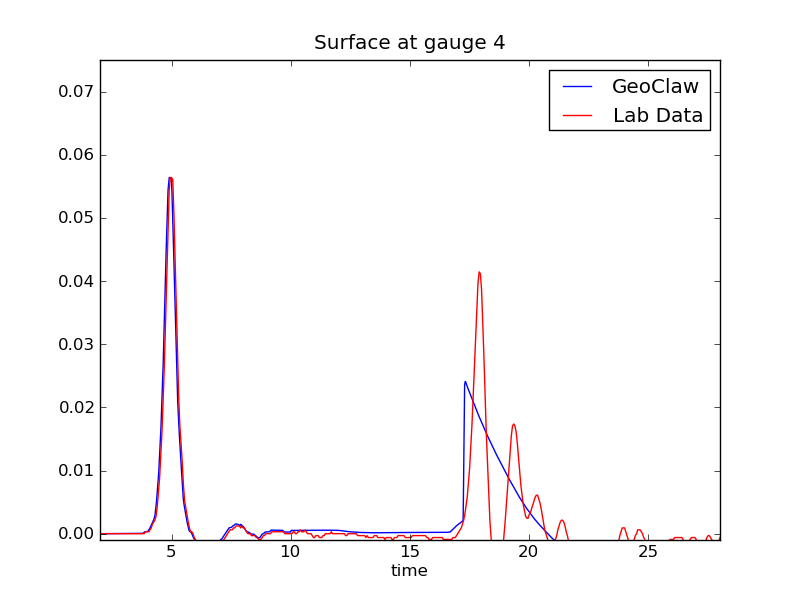
\includegraphics[width=2.8in]{bp5/CaseB/gauge0004fig300.png}\hfil
\hfil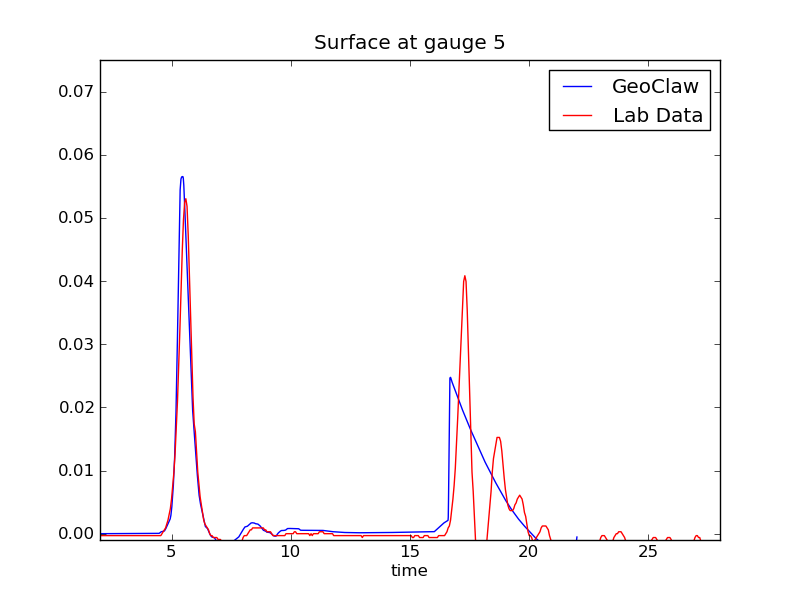
\includegraphics[width=2.8in]{bp5/CaseB/gauge0005fig300.png}\hfil
\vskip 5pt
\hfil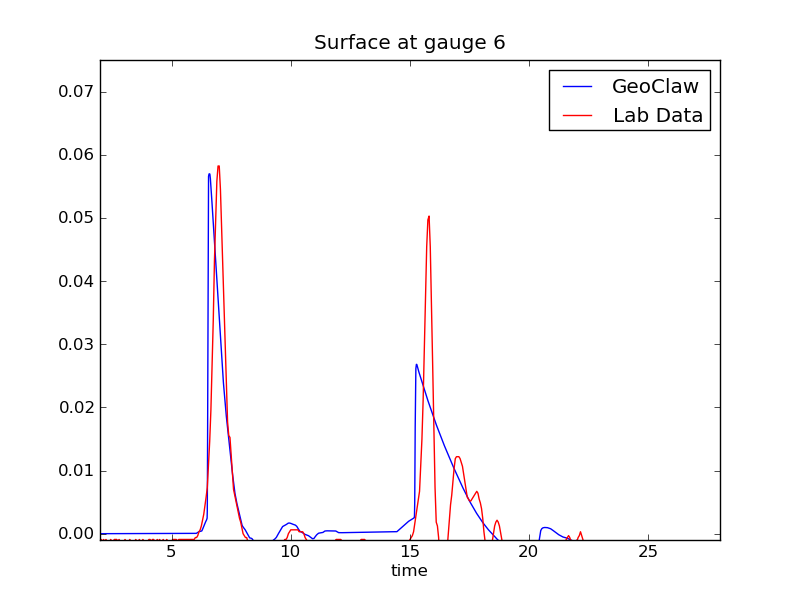
\includegraphics[width=2.8in]{bp5/CaseB/gauge0006fig300.png}\hfil
\hfil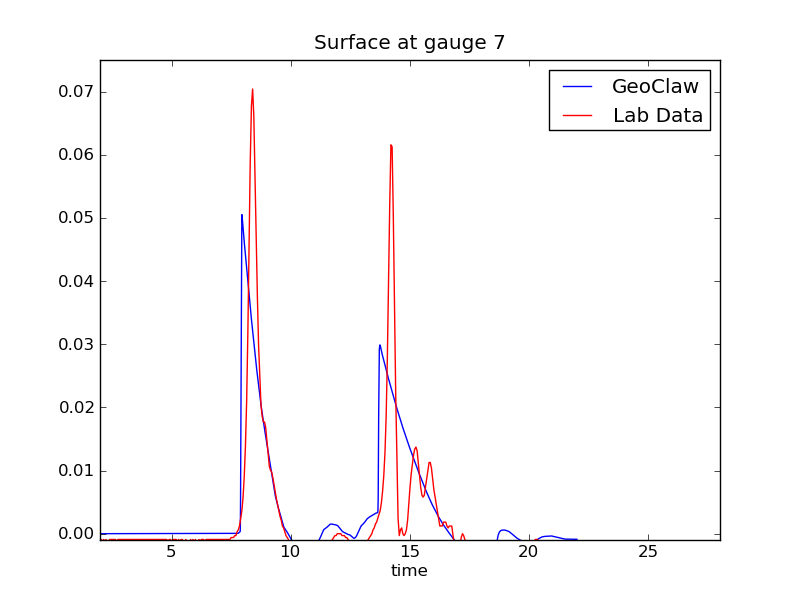
\includegraphics[width=2.8in]{bp5/CaseB/gauge0007fig300.png}\hfil
\vskip 5pt
\hfil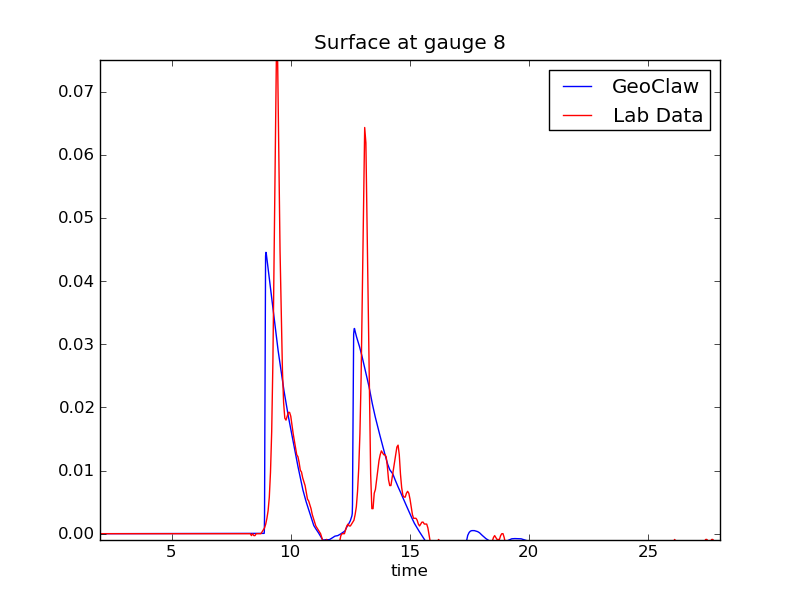
\includegraphics[width=2.8in]{bp5/CaseB/gauge0008fig300.png}\hfil
\hfil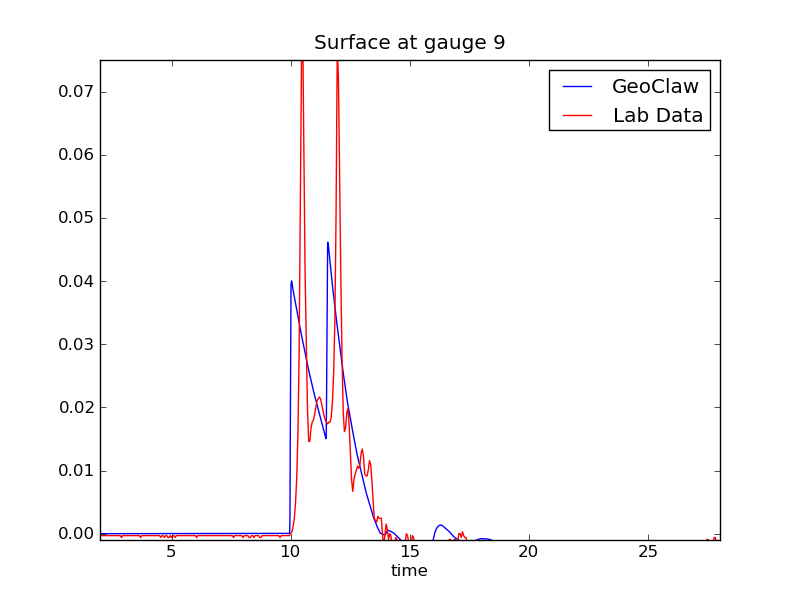
\includegraphics[width=2.8in]{bp5/CaseB/gauge0009fig300.png}\hfil
\vskip 5pt
\hfil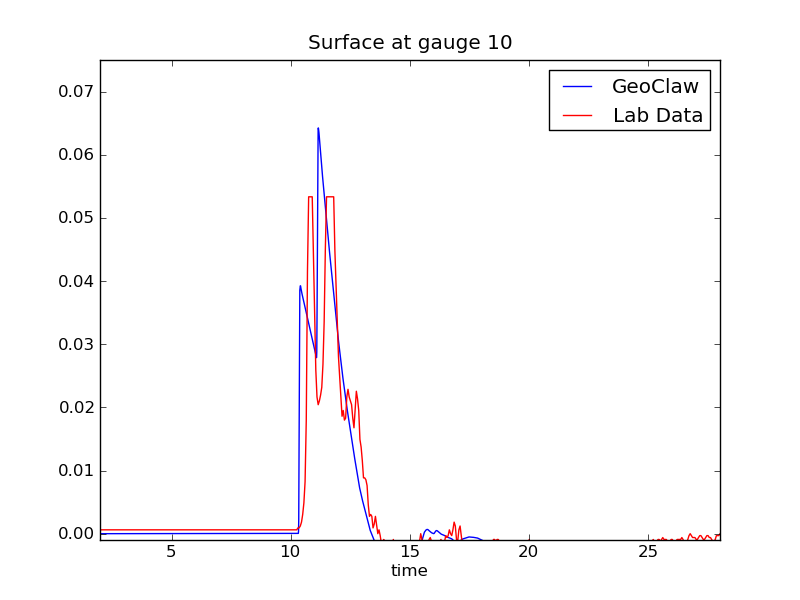
\includegraphics[width=2.8in]{bp5/CaseB/gauge0010fig300.png}\hfil
\hfil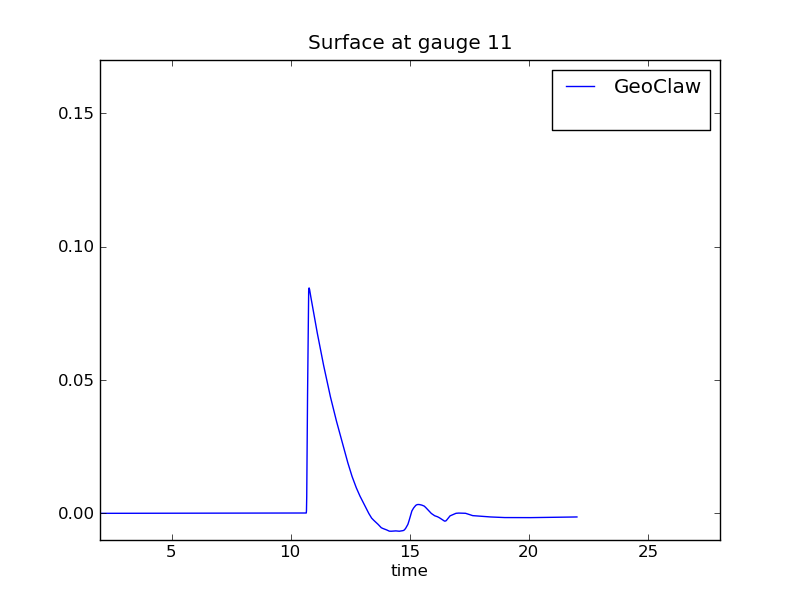
\includegraphics[width=2.8in]{bp5/CaseB/gauge0011fig300.png}\hfil
\caption{\label{fig:bp5B} Case B }
\end{figure}

\begin{figure}[ht]
\hfil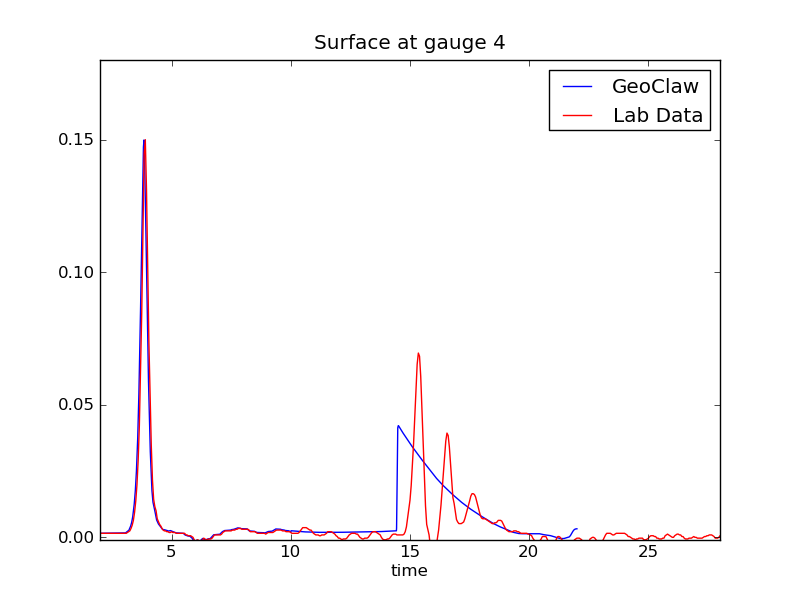
\includegraphics[width=2.8in]{bp5/CaseC/gauge0004fig300.png}\hfil
\hfil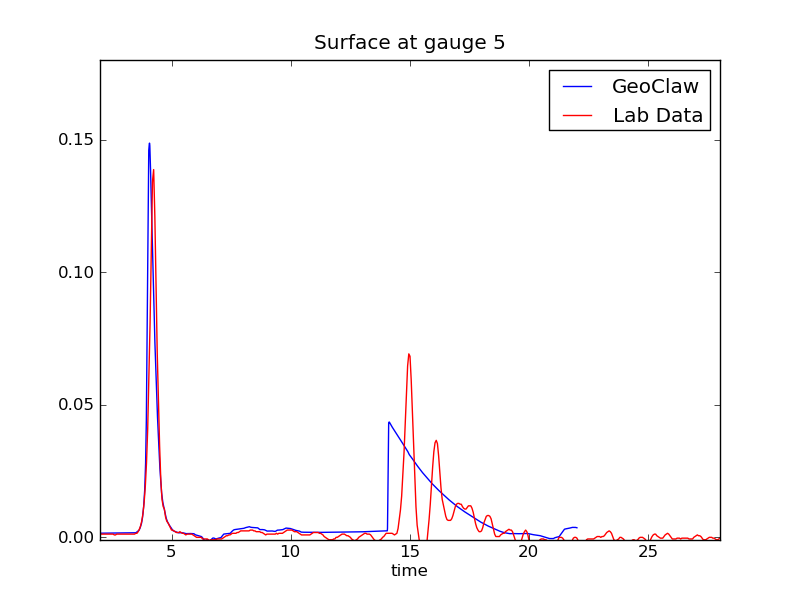
\includegraphics[width=2.8in]{bp5/CaseC/gauge0005fig300.png}\hfil
\vskip 5pt
\hfil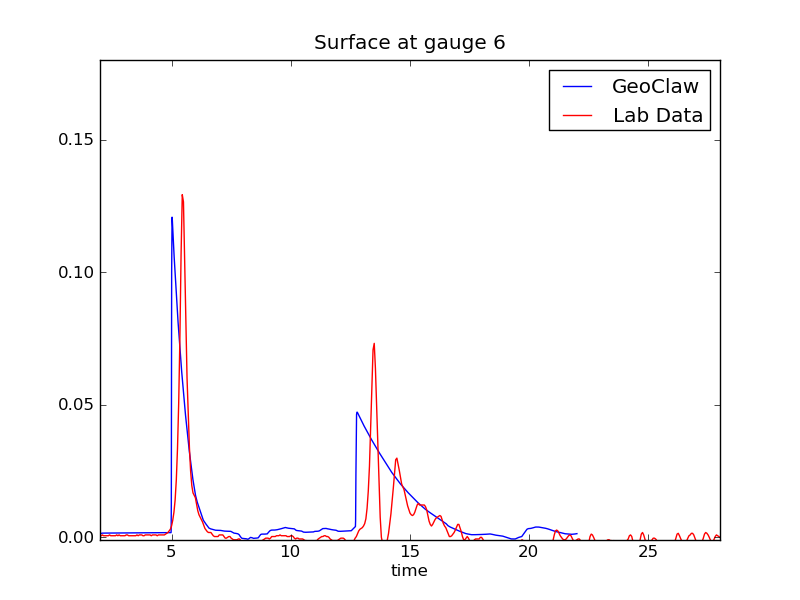
\includegraphics[width=2.8in]{bp5/CaseC/gauge0006fig300.png}\hfil
\hfil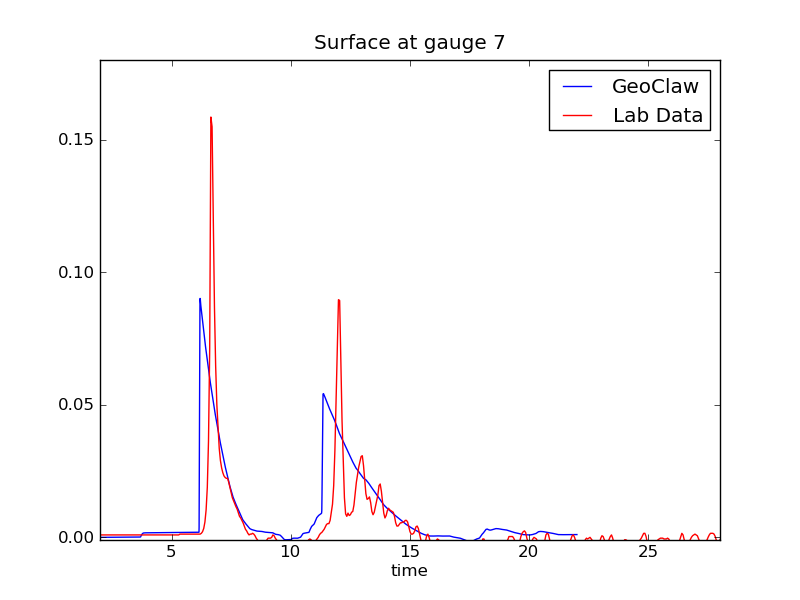
\includegraphics[width=2.8in]{bp5/CaseC/gauge0007fig300.png}\hfil
\vskip 5pt
\hfil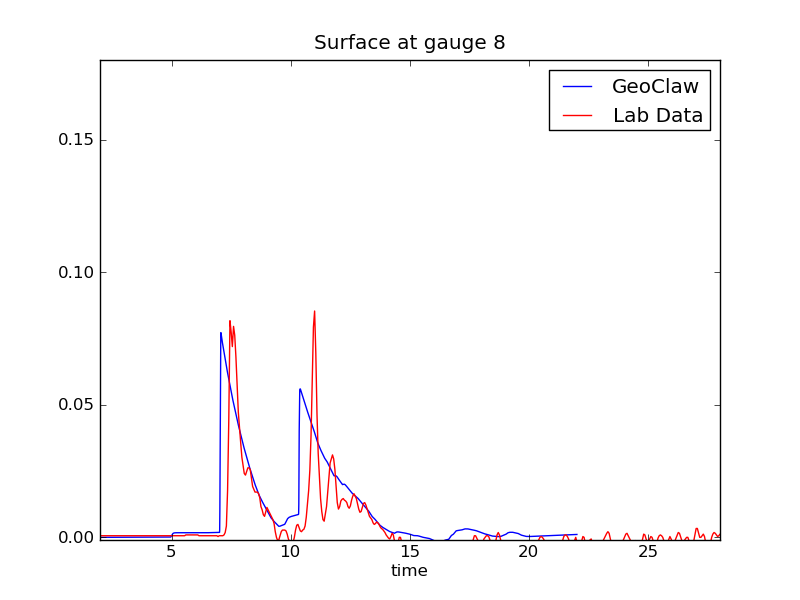
\includegraphics[width=2.8in]{bp5/CaseC/gauge0008fig300.png}\hfil
\hfil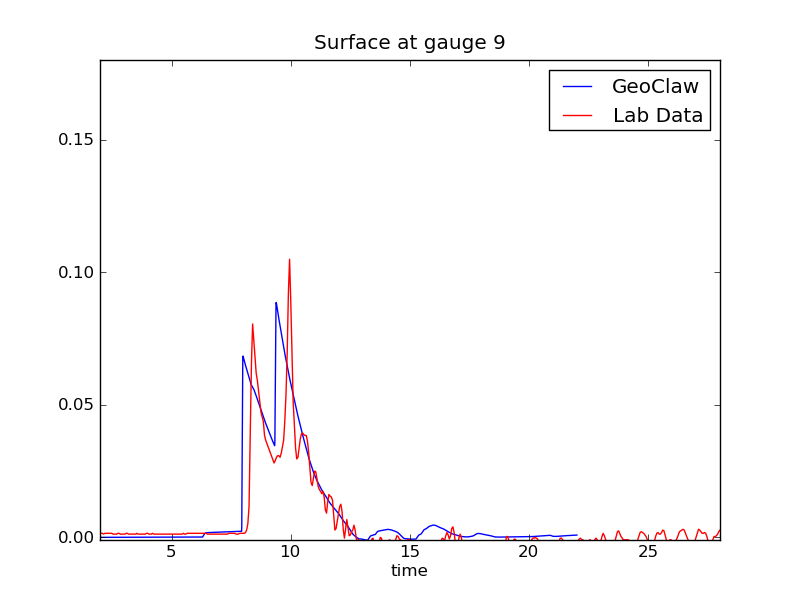
\includegraphics[width=2.8in]{bp5/CaseC/gauge0009fig300.png}\hfil
\vskip 5pt
\hfil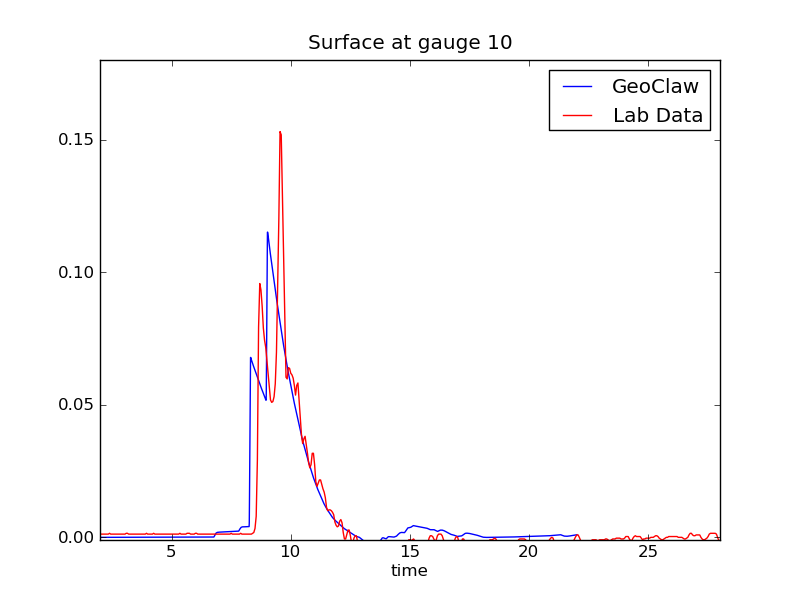
\includegraphics[width=2.8in]{bp5/CaseC/gauge0010fig300.png}\hfil
\hfil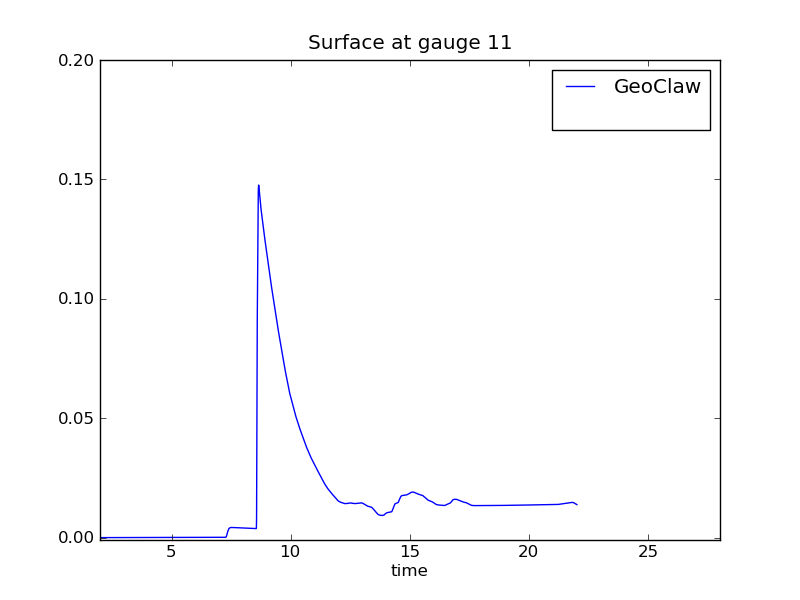
\includegraphics[width=2.8in]{bp5/CaseC/gauge0011fig300.png}\hfil
\caption{\label{fig:bp5C} Case C }
\end{figure}

\subsubsection{Convergence Study}
We performed a test to see how well Clawpack converged to the gage measurements as we increased the number of grid cells in our computational domain.  We found that as the number of grid cells was increased that the computed solution converged and had a shock in approximately the same location as in the gage data.  The results shown in figure \Fig{nonLinearConverge}.

\begin{figure}[ht]
\hfil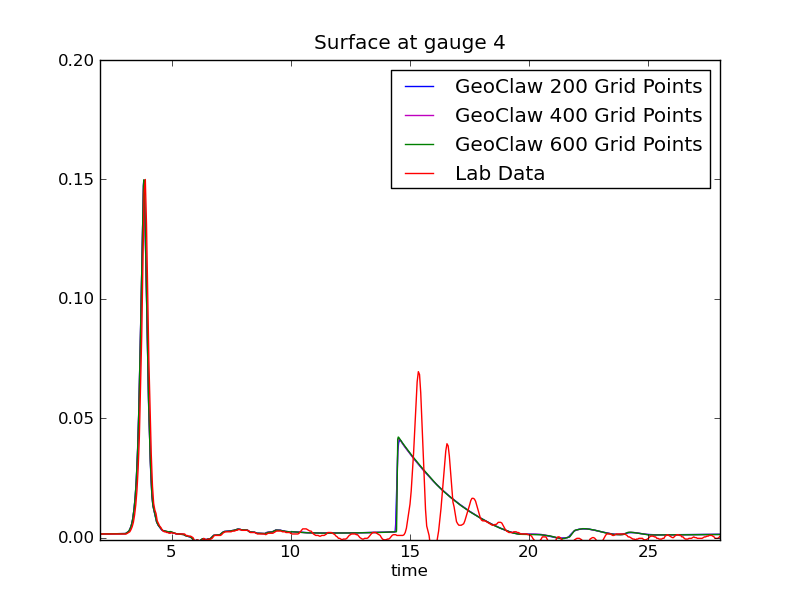
\includegraphics[width=5in]{bp5/nonLinearCompare}\hfil
\caption{\label{fig:nonLinearConverge} Convergence Plot for Gage 4 in Case C }
\end{figure}

\subsubsection{Lessons learned}
In this benchmark problem we found that using the measured data from Gage 4 as boundary conditions on a shorter domain, starting at this Gage, provided more accurate results than using the wave maker position and a longer domain to model the entire tank.  It appears that a similar assumption is made in the provided analytic solutions, as they match up nearly perfectly with the lab data for the first ten seconds.  

Overall this benchmark problem is a good test for one dimensional codes.  
Case C exhibits dispersion in the laboratory results not seen with the
nonlinear shallow water equations.

The benchmark problem specifications could be improved by specifying the computational domain and the specific data source that should be used to model the incoming wave. 
